\documentclass[11pt]{article}

\usepackage[T1]{fontenc}
\usepackage[utf8]{inputenc}
\usepackage{lmodern}
\usepackage{microtype}
\usepackage[margin=0.84in]{geometry}
\usepackage{amsmath,amssymb,amsthm}
\usepackage{booktabs,tabularx,array}
\usepackage{graphicx}
\usepackage{caption}
\usepackage{enumitem}
\usepackage{xcolor}
\usepackage[numbers,sort&compress]{natbib}
\usepackage{hyperref}
\usepackage{titlesec}
\usepackage{fancyhdr}

\definecolor{deepblue}{HTML}{194F70}
\definecolor{teal}{HTML}{2F7D6D}
\definecolor{softgray}{HTML}{F3F5F7}
\definecolor{rulegray}{HTML}{CBD5DC}
\hypersetup{colorlinks=true,linkcolor=deepblue,citecolor=deepblue,urlcolor=deepblue,pdfauthor={},pdftitle={Bulk tissue nitrite alone does not identify eNOS/iNOS source contributions},pdfsubject={Partial-identification audit of published aggregate nitrite data}}
\graphicspath{{../../evidence/}}
\setlength{\parindent}{0pt}
\setlength{\parskip}{0.58em}
\setlist{nosep,leftmargin=1.5em}
\captionsetup{font=small,labelfont=bf}
\titleformat{\section}{\large\bfseries\color{deepblue}}{\thesection}{0.6em}{}
\titleformat{\subsection}{\normalsize\bfseries}{\thesubsection}{0.55em}{}
\pagestyle{fancy}
\fancyhf{}
\fancyhead[L]{\small Source identification from bulk nitrite}
\fancyfoot[C]{\thepage}
\renewcommand{\headrulewidth}{0.4pt}
\fancypagestyle{plain}{
  \fancyhf{}
  \fancyhead[L]{\small Source identification from bulk nitrite}
  \fancyfoot[C]{\thepage}
  \renewcommand{\headrulewidth}{0.4pt}
}
\fancypagestyle{titlepage}{
  \fancyhf{}
  \fancyfoot[C]{\thepage}
  \renewcommand{\headrulewidth}{0pt}
}
\newtheorem{theorem}{Theorem}
\newtheorem{corollary}{Corollary}
\newtheorem{proposition}{Proposition}
\newcommand{\ASEO}{\textit{Allium sativum} essential oil}
\newcommand{\Rplus}{\mathbb{R}_{\geq 0}}

\title{\vspace{-1.5em}\textbf{Bulk tissue nitrite alone does not identify\\[-0.05em]eNOS/iNOS source contributions:}\\[0.25em]
\large A partial-identification audit of garlic-oil responses under lead exposure}
\author{}
\date{24 August 2026}

\begin{document}
\maketitle
\thispagestyle{titlepage}

\begin{abstract}
Two publicly unlinked mouse reports using lead nitrate and garlic essential oil described higher cardiac and lower renal tissue-homogenate nitrite in the high-dose group. The reported lead-plus-olive-oil groups serve only as nominal vehicle references; causal comparability is not assumed. We audited provenance, reconstructed an unadjusted aggregate heart contrast, and performed an exact tissue-specific partial-identification analysis. In a deliberately favorable model, each tissue total is a nonnegative weighted sum of effective eNOS- and iNOS-attributed contributions. The sharp interval for a high-dose-minus-reference source contrast is $[-y_0/a_k,y_1/a_k]$. It contains both signs for every $y_0,y_1>0$: the numerical observations determine interval endpoints, not the qualitative impossibility. The reported values give $[-2.24,6.29]$ in heart and $[-1.43,0.7162]$ in kidney for either unit-response component. Strictly positive tissue-specific allocations reproduce each pair of means while reversing the heart-eNOS and kidney-iNOS target signs. Thus these bulk observations identify neither source level nor source-effect sign, but they also do not falsify the biological hypothesis. Executable certificates, external-fraction sensitivity bounds, and a prospective pathway-coherence design framework specify what additional restrictions or experiments would be needed; literal pool partition requires a validated source-selective measurement.
\end{abstract}

\noindent\textbf{Keywords:} nitric oxide; nitrite; identifiability; partial identification; eNOS; iNOS; lead; garlic essential oil; vascular function; nephrotoxicity

\begin{center}
\fcolorbox{rulegray}{softgray}{\begin{minipage}{0.92\textwidth}
\textbf{Claim status.} This paper reports a formal result and an audit of published group-level values. It contains no new animal observations. The mechanistic biological hypothesis remains untested; the negative result concerns what can be inferred from the existing bulk measurements.
\end{minipage}}
\end{center}

\section{Introduction}

Nitric oxide (NO) biology is defined as much by source, location, redox state, and consumption as by the abundance of stable downstream metabolites. Because NO is short lived, nitrite and nitrate are often used as practical indices. Those measurements can be informative, but extrapolation from a sampled metabolite pool to a tissue-specific source requires additional assumptions and validation \citep{bryan2007,giustarini2008}. In lead toxicity this distinction is especially important: lead-associated reactive oxygen species can reduce NO bioavailability while NOS abundance or measured NO metabolites increase compensatorily \citep{vaziri1999,vaziri2001,silveira2014}. An abundance measurement, a catalytic flux, and a downstream functional response are therefore different estimands.

Rajpoot and Sharma reported that high-dose \ASEO{} increased cardiac-homogenate nitrite in lead-nitrate-exposed male Swiss albino mice \citep{rajpoot2025}. A separate renal study reported a decrease under a similar nominal treatment regime \citep{sharma2024}. Garlic-derived compounds provide biological motivation for differential regulation: cell-system experiments have reported suppression of inflammatory iNOS expression and enhancement or protection of endothelial NO/cGMP signaling \citep{kim2001,lei2010}. Yet those studies involve different preparations, systems, and estimands. They do not turn bulk tissue nitrite into an isoform-specific measurement.

The target mechanistic hypothesis is that high-dose \ASEO{} restores a coupled eNOS--soluble-guanylate-cyclase (sGC)--cGMP axis in the cardiovascular system while reducing renal NOS2-linked nitrative stress. A directional heart-up/kidney-down nitrite pattern is compatible with that hypothesis. Compatibility, however, is weaker than identification. Here we ask a precise question: \emph{what source-level conclusions are logically determined by the reported bulk means?}

Our contributions are application specific. We (i) preserve and audit the published aggregate values; (ii) derive sharp source-effect bounds under a favorable nonnegative additive model; (iii) provide explicit, strictly positive source-reversal certificates; (iv) quantify how external source-fraction bounds could identify a sign; (v) separate sampling precision of the bulk contrast from structural identification of latent sources; and (vi) distinguish causal pathway contribution and mechanistic coherence from literal pool partition. This analysis follows the partial-identification distinction between what data and assumptions determine and what remains set identified \citep{tamer2010,imbensmanski2004}. The row-space criterion is classical estimability; its value here is to expose exactly what these observations do and do not determine \citep{searle1971}.

\section{Materials and methods}

\subsection{Source records and data provenance}

The cardiac source is a six-group mouse report ($n=6$ per group) presenting nitrite as mean $\pm$ standard error of the mean (SEM) in nmol/mL of 10\% heart homogenate \citep{rajpoot2025}. The renal source is a separate six-group publication ($n=6$ per group) reporting ``NO'' means in $\mu$mol/L from 10\% renal homogenate; numeric uncertainty is shown graphically but not printed \citep{sharma2024}. Because
\[
1\ \mu\mathrm{mol/L}=1\ \mathrm{nmol/mL},
\]
the numeric concentration scales are dimensionally identical. They are not thereby biologically comparable or pairable. The publications provide no animal identifiers that permit cohort linkage, and they do not document a shared oil batch or harmonized processing beyond the nominal kit and 10\% homogenate description. We therefore treat the reports as publicly unlinked; we do not assume either independence or reuse.

Values were transcribed without graph-digitizing missing error bars and stored in a machine-readable table. No individual-animal observations, calibration curves, plate layouts, or raw instrument files were available. All derived calculations therefore operate on published aggregates and are labeled as such. Table~\ref{tab:provenance} summarizes the quotation-level audit; exact locations, short source excerpts, competing duration readings, and their consequences are archived in the accompanying provenance record.

\begin{table}[htbp]
\centering
\caption{Source-provenance fields material to the descriptive contrast. ``Not reported'' means not located in the cited report, not that the procedure did not occur.}
\label{tab:provenance}
\scriptsize
\begin{tabularx}{\textwidth}{>{\raggedright\arraybackslash}p{0.19\textwidth}>{\raggedright\arraybackslash}p{0.37\textwidth}X}
\toprule
Field & Cardiac report & Renal report \\
\midrule
Reported groups & Group IV, lead nitrate + high-dose ASEO; Group VI, lead nitrate + ``Vehicle control (Olive oil)'' & Group IIc, lead nitrate + high-dose garlic oil; Group IIe, lead nitrate + vehicle olive oil \\
Lead route/frequency & Not reported / not reported & Oral gavage / frequency not reported \\
ASEO route/frequency & Not reported / not reported & Oral gavage / frequency not reported \\
Vehicle identity/volume & Olive oil; dose and volume not reported & ASEO prepared in olive oil; vehicle dose and volume not reported \\
Schedule & Methods: 30-day study, adjuncts day 12 to end; abstract can instead read as 12 days followed by 30 treatment days & Lead for 30 days; adjuncts day 12 to end \\
Assay/kit & Elabscience E-BC-K035-M; absorbance 550 nm; nitrite standard curve & Elabscience E-BC-K035-M colorimetric kit; wavelength/standard details not stated \\
Reported analyte & NO indirectly quantified through nitrite & Labeled NO; direct chemical readout not specified \\
Preparation and normalization & 10\% w/v homogenate supernatant; concentration only, no wet-mass/protein normalization & 10\% w/v homogenate supernatant; concentration only, no wet-mass/protein normalization \\
Nitrate reduction/deproteinization & Neither reported & Neither reported \\
\bottomrule
\end{tabularx}
\end{table}

The shared catalog number does not prove equivalent recovery across tissues or reports. Neither report validates direct lead-nitrate matrix interference. Lead nitrate may affect biological nitrate--nitrite handling, but any direct analytical interference remains unknown rather than assumed.

\subsection{Observed contrasts}

The primary descriptive comparison is high-dose ASEO versus the reported lead-plus-olive-oil group, used as a nominal vehicle reference. Causal comparability and an isolated oil effect are not asserted. The report-nominated high-dose-versus-lead-alone comparison is retained as secondary. Using the rounded published means and SEMs as reported, and assuming the SEMs summarize independent animals rather than technical replicates, we computed unadjusted approximate two-group Welch intervals for heart. Rounding error in the published SEMs is ignored. If $\bar y_1, s_{\bar y_1}$ and $\bar y_0, s_{\bar y_0}$ denote group means and SEMs, then
\[
\widehat{\Delta}=\bar y_1-\bar y_0,\qquad
\mathrm{SE}(\widehat{\Delta})=\sqrt{s_{\bar y_1}^2+s_{\bar y_0}^2},
\]
with Welch--Satterthwaite degrees of freedom. These intervals are unadjusted despite the source report's six groups, ignore any technical-replicate structure, and do not reconstruct its multiple-group analysis. They describe sampling uncertainty only under the stated assumptions and do not solve the source-identification problem. No renal confidence interval was calculated because numeric renal SEMs were unavailable.

\subsection{Effective-source model}

Let $g\in\{0,1\}$ denote a stated reference and lead plus high-dose ASEO, and let $t\in\{\mathrm{heart},\mathrm{kidney}\}$ index tissue/report. The primary application uses the reported lead-plus-olive-oil group as the nominal reference; the report-nominated lead-alone contrast is secondary. For each tissue separately, let
\[
y_{gt}=A_t x_{gt},\qquad x_{gt}\in\Rplus^p,
\]
where $y_{gt}\in\mathbb R^{m_t}$ contains exact bulk measurements, $A_t\in\mathbb R^{m_t\times p}_{\geq0}$ is condition invariant within tissue, and $x_{gt}$ contains nonnegative \emph{effective contributions to the measured analyte}. We assume neither $A_{\mathrm{heart}}=A_{\mathrm{kidney}}$, nor a common latent-source scale, nor a joint animal-level distribution. The juxtaposition of organs is biological motivation, not a statistically combined cross-organ estimand. This semantic boundary is essential: without an independently validated map, coordinates of $x_{gt}$ are not NOS protein abundance, catalytic activity, instantaneous NO synthesis, or vascular function.

For the two-source illustration,
\[
y_{gt}=a_{tE} x_{gtE}+a_{tI} x_{gtI},\qquad a_{tE},a_{tI}>0,
\]
where $E$ and $I$ label eNOS- and iNOS-attributed contributions. Defining $u_{gtk}=a_{tk}x_{gtk}$ gives $y_{gt}=u_{gtE}+u_{gtI}$ within each tissue. This model is intentionally favorable to source partition: it omits nNOS, NOS-independent nitrite reduction, diet and microbiome inputs, blood contamination, nitrate--nitrite exchange, spatial transport, clearance, chemical consumption, and condition-dependent recovery. Failure of identification inside this restricted model defeats identification from the bulk totals alone; unmeasured additions cannot restore it without new restrictions.

For any source functional $c^\top x$, define the feasible set and its linear-program bounds \citep{boydvandenberghe2004}
\[
\mathcal F_A(y)=\{x\in\Rplus^p:Ax=y\},\qquad
L_c(y)=\min_{x\in\mathcal F_A(y)}c^\top x,\quad
U_c(y)=\max_{x\in\mathcal F_A(y)}c^\top x.
\]

\subsection{Computation, tests, and literature boundary}

Deterministic Python code transcribes no latent animal data and uses no random numbers. It checks the unit conversion; reconstructs published totals from explicit source allocations; verifies positivity and sign reversal; calculates sharp intervals, matrix ranks, and aggregate heart intervals; and creates figures and a prospective standardized-effect power sensitivity grid. Automated tests assert the reported numerical certificates. The bounded search record documents database-specific queries and primary method/mechanism sources through 24 August 2026. It was designed for evidence retrieval, not a systematic review, and supports no novelty or priority claim.

\section{Results}

\subsection{Published bulk directions}

Table~\ref{tab:published} gives the complete six-group transcription from each report; Figure~\ref{fig:bulk} displays the four groups used to motivate the source audit. Cardiac nitrite fell under lead and was higher with high-dose ASEO; renal nitrite rose under lead and was lower with high-dose ASEO. The nominal vehicle-referenced descriptive differences are heart $6.29-2.24=+4.05$ nmol/mL and kidney $0.7162-1.43=-0.7138$ $\mu$mol/L. Under the approximate unadjusted analysis and its independence assumptions, the heart aggregate contrast has an interval excluding zero: SE $0.243$, $\nu=5.28$, and 95\% CI $[3.43,4.67]$. The secondary high-dose-minus-lead contrast was $+4.91$ nmol/mL (SE $0.253$, $\nu=6.10$, unadjusted 95\% CI $[4.29,5.53]$). Neither result identifies a latent source contrast. Neither report includes an ASEO-only group.

\begin{table}[htbp]
\centering
\caption{Complete six-group transcription of published tissue-homogenate values labeled nitrite/NO. Heart values are mean $\pm$ SEM; renal numeric SEMs were not printed. Animal-level linkage is unavailable.}
\label{tab:published}
\begin{tabular}{lcc}
\toprule
Group & Heart (nmol/mL) & Kidney ($\mu$mol/L) \\
\midrule
Control & $10.43\pm0.14$ & 1.25 \\
Lead & $1.38\pm0.08$ & 2.022 \\
Lead + ASEO, 50 mg/kg & $1.82\pm0.10$ & 1.1216 \\
Lead + ASEO, 80 mg/kg & $6.29\pm0.24$ & 0.7162 \\
Lead + silymarin, 25 mg/kg & $2.00\pm0.04$ & 0.6711 \\
Lead + olive oil & $2.24\pm0.04$ & 1.43 \\
\bottomrule
\end{tabular}
\end{table}

\begin{figure}[htbp]
\centering
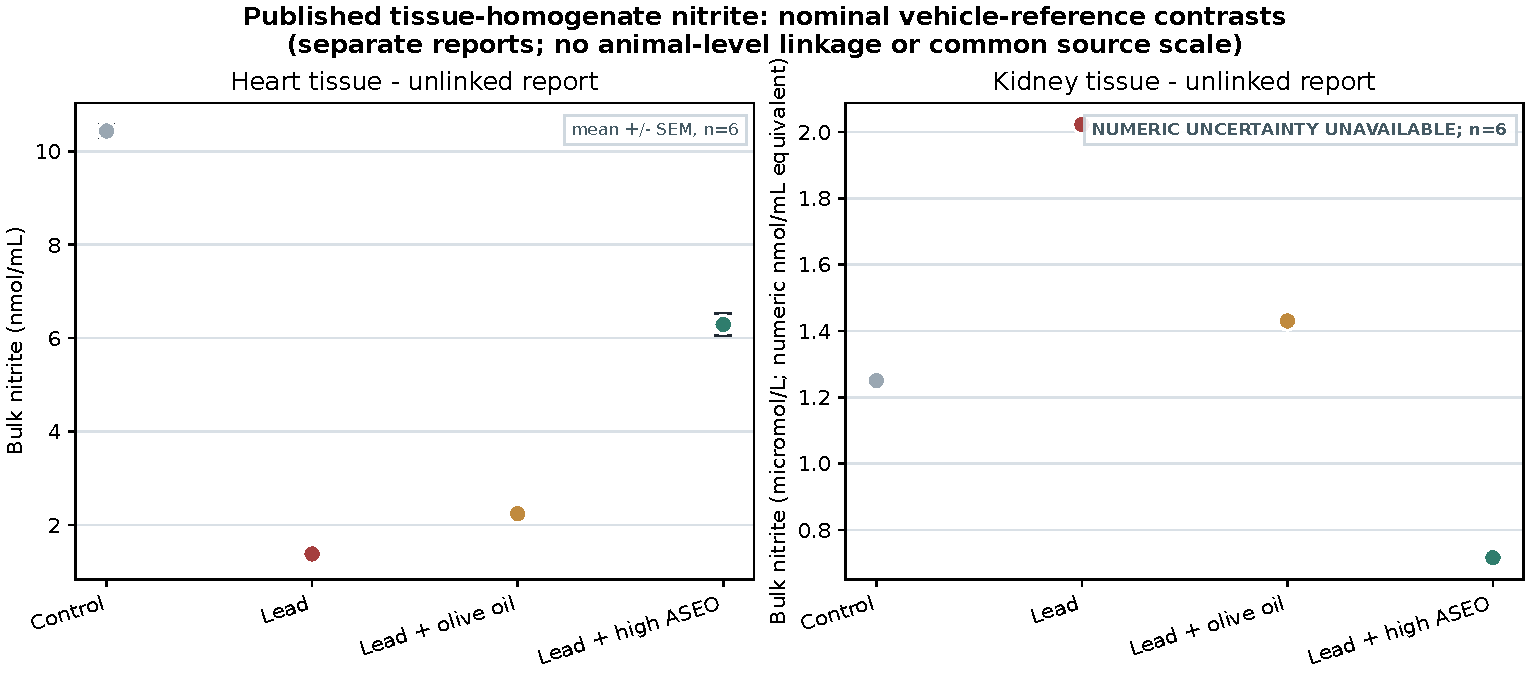
\includegraphics[width=0.98\textwidth]{published_bulk_directions.pdf}
\caption{Selected published tissue-homogenate observations in separate cardiac and renal reports \citep{rajpoot2025,sharma2024}. Points and numeric intervals are shown only where SEMs were printed. The renal axis preserves the source unit. Side-by-side panels do not imply cohort linkage, exchangeability, or a common biological scale.}
\label{fig:bulk}
\end{figure}

\newpage
\thispagestyle{fancy}
\subsection{Sharp contrast bounds}

\begin{theorem}[Exact contrast interval]
Suppose the two conditions are constrained only by $x_g\in\mathcal F_A(y_g)$, with no cross-condition coupling constraints, and the extrema are finite and attained. Then the identified set for the condition contrast $c^\top(x_1-x_0)$ is exactly
\[
\left[L_c(y_1)-U_c(y_0),\ U_c(y_1)-L_c(y_0)\right].
\]
\end{theorem}

\begin{proof}
Each feasible set is convex, so its image under the linear map $x\mapsto c^\top x$ is an interval, namely $[L_c(y_g),U_c(y_g)]$. Conditions are otherwise unrestricted, so any feasible value in the treated interval can be paired with any feasible value in the baseline interval. Subtracting the intervals gives the displayed bounds. Selecting a treated minimizer and baseline maximizer attains the lower endpoint; selecting a treated maximizer and baseline minimizer attains the upper endpoint. Hence the bounds are sharp.
\end{proof}

The corresponding linear-program duals are
\[
L_c(y)=\max_{\lambda:A^\top\lambda\leq c}\lambda^\top y,
\qquad
U_c(y)=\min_{\lambda:A^\top\lambda\geq c}\lambda^\top y,
\]
under standard primal/dual feasibility conditions \citep{boydvandenberghe2004}. These forms allow extra calibrated assays and defensible bounds to be incorporated without pretending that missing latent values were observed.

\begin{corollary}[One positive bulk total]
For one fixed tissue $t$, let $y_{gt}=a_{tE}x_{gtE}+a_{tI}x_{gtI}$ with $a_{tE},a_{tI}>0$. The sharp high-dose-minus-reference interval for source $k\in\{E,I\}$ is
\[
\Delta x_{tk}\in\left[-\frac{y_{0t}}{a_{tk}},\frac{y_{1t}}{a_{tk}}\right].
\]
When both totals are positive, negative, zero, and positive source contrasts are all compatible with that tissue's observations.
\end{corollary}

\begin{proof}
For a fixed condition, nonnegativity and the single equality give $x_{gtk}\in[0,y_{gt}/a_{tk}]$; every point in that interval is feasible by assigning the remainder to the other positive source. The theorem then gives the contrast interval. Under nonnegativity the endpoints are closed and attained. With strict positivity they are open limits, while every interior sign remains feasible.
\end{proof}

The qualitative impossibility is data independent within this model: every $y_{0t},y_{1t}>0$ yields an interval containing both signs. The reported values determine only the endpoints. In weighted units ($a_{tk}=1$ after absorption into $u_{gtk}$), the nominal vehicle-referenced heart interval is $[-2.24,6.29]$ nmol/mL for either source; the kidney interval is $[-1.43,0.7162]$ $\mu$mol/L for either source. For tissue $t$, the joint identified set is the bounded line segment
\[
\left\{(\Delta u_{tE},\Delta u_{tI}):\ \Delta u_{tE}+\Delta u_{tI}=y_{1t}-y_{0t},\quad
\Delta u_{tE},\Delta u_{tI}\in[-y_{0t},y_{1t}]\right\}.
\]
Accordingly, the nominal-reference sums are $\Delta u_{\mathrm{heart},E}+\Delta u_{\mathrm{heart},I}=4.05$ and $\Delta u_{\mathrm{kidney},E}+\Delta u_{\mathrm{kidney},I}=-0.7138$. A positive heart sum implies that at least one weighted source rose, but not which one; the negative renal sum implies that at least one fell, but not which one. The secondary lead-alone intervals, $[-1.38,6.29]$ and $[-2.022,0.7162]$, also contain both signs.

\begin{proposition}[External source-fraction sensitivity]
For a fixed tissue and source $k$, suppose externally validated information bounds the weighted source fraction as $f_{gk}=u_{gk}/y_g\in[\ell_{gk},r_{gk}]$, independently across conditions. Then the sharp source-contrast interval is
\[
\Delta u_k\in[\ell_{1k}y_1-r_{0k}y_0,\ r_{1k}y_1-\ell_{0k}y_0].
\]
A positive sign is identified if $\ell_{1k}y_1>r_{0k}y_0$; a negative sign is identified if $r_{1k}y_1<\ell_{0k}y_0$.
\end{proposition}

The result follows by taking the independent interval difference. When the denominator bounds are positive, heart-positive eNOS attribution requires $\ell_{1E}/r_{0E}>0.3561$, and kidney-negative iNOS attribution requires $\ell_{0I}/r_{1I}>0.5008$. These are transparent requirements on external information, not estimates from the bulk observations.

\subsection{Exact source-reversal certificates}

Table~\ref{tab:witnesses} gives two sets of tissue-specific logical allocations, displayed together for convenience. They do not describe linked animals. Each row sums exactly to the corresponding published mean. Allocation A gives the proposed heart-eNOS and kidney-iNOS target signs; Allocation B reverses only the interpretive conclusion under audit. The unhighlighted coordinate in each row is a balance term required by the two-component illustration, not an additional target hypothesis. Each organ separately fails to identify either source-effect sign (Figure~\ref{fig:witnesses}).

\begin{table}[htbp]
\centering
\caption{Strictly positive tissue-specific allocations reproducing the nominal-reference and high-dose means. Boldface marks the coordinate under audit. Values are weighted effective contributions, not enzyme fluxes.}
\label{tab:witnesses}
\small
\begin{tabularx}{\textwidth}{>{\raggedright\arraybackslash}p{0.14\textwidth}lcc>{\raggedright\arraybackslash}p{0.19\textwidth}>{\raggedright\arraybackslash}X}
\toprule
Allocation & Tissue & Nominal reference & High ASEO & Audited coordinate & Contrast $(\Delta u_E,\Delta u_I)$ \\
\midrule
A: target & Heart & $(0.10,2.14)$ & $(6.19,0.10)$ & $\Delta u_E$ & $(\mathbf{+6.09},-2.04)$ \\
A: target & Kidney & $(0.10,1.33)$ & $(0.6162,0.10)$ & $\Delta u_I$ & $(+0.5162,\mathbf{-1.23})$ \\
B: reversed & Heart & $(2.14,0.10)$ & $(0.10,6.19)$ & $\Delta u_E$ & $(\mathbf{-2.04},+6.09)$ \\
B: reversed & Kidney & $(1.33,0.10)$ & $(0.10,0.6162)$ & $\Delta u_I$ & $(-1.23,\mathbf{+0.5162})$ \\
\bottomrule
\end{tabularx}
\end{table}

\begin{figure}[htbp]
\centering
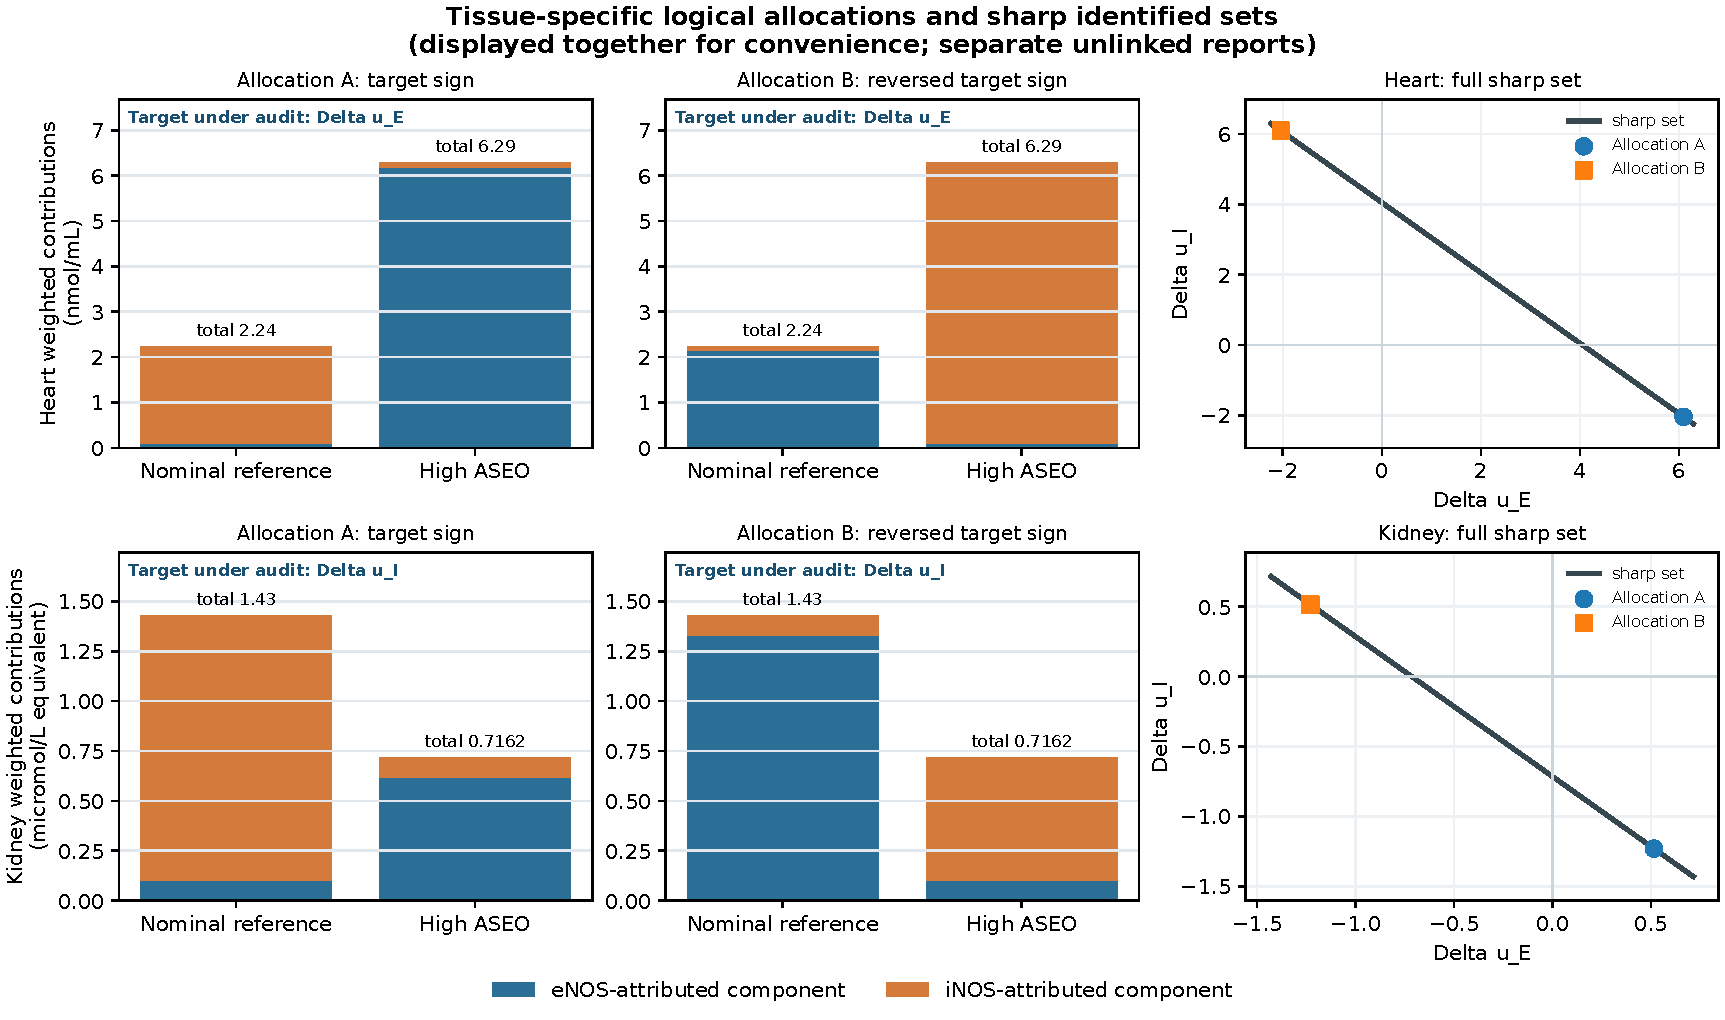
\includegraphics[width=0.98\textwidth]{source_partition_witnesses.pdf}
\caption{Tissue-specific logical certificates and the entire sharp line segment for each tissue. Independent tissue scales prevent visual cross-organ comparison. The panels are juxtaposed for convenience and do not represent linked animals or a common source scale.}
\label{fig:witnesses}
\end{figure}

\clearpage
\thispagestyle{fancy}
Treating each positive sample mean as exact isolates the structural question. Standard errors, narrower confidence intervals, more animals, or a smaller p-value for the same total measurement do not select a source allocation. Allowing each total to vary over a validated positive measurement interval retains sign nonidentification absent additional coupling or fraction restrictions.

\subsection{When an added measurement identifies a source}

For the exact, known, linear model $y=Ax$ in which every row measures the same latent vector, call $c^\top x$ \emph{globally identified} if, for all interior states $x,x'\gg0$, $Ax=Ax'$ implies $c^\top x=c^\top x'$.

\begin{theorem}[Global row-space criterion]
Under that definition, $c^\top x$ is globally point identified if and only if $c$ lies in the row space of $A$ \citep{searle1971}.
\end{theorem}

\begin{proof}
If $c\in\operatorname{Row}(A)$, then $c=A^\top\lambda$ for some $\lambda$, so $c^\top x=\lambda^\top Ax=\lambda^\top y$ is fixed by the observation. Conversely, if $c\notin\operatorname{Row}(A)$, the fundamental theorem of linear algebra gives $h\in\ker(A)$ with $c^\top h\neq0$. Choose an interior state $x\gg0$. For sufficiently small $\varepsilon>0$, both $x+\varepsilon h$ and $x-\varepsilon h$ remain interior and yield the same $y$, but their functional values differ. Hence global point identification fails.
\end{proof}

For an exceptional fixed observation, the computational condition is $L_c(y)=U_c(y)$. For a condition contrast with condition-specific matrices, global identification requires $c\in\operatorname{Row}(A_0)\cap\operatorname{Row}(A_1)$. After adding calibrated measurement rows $B$, the source functional becomes identified exactly when
\[
c\in\operatorname{Row}\!\begin{pmatrix}A\\B\end{pmatrix};
\]
the complete latent vector requires full column rank. In a closed two-source system, a second row $b=(b_E,b_I)$ complements the bulk row $a=(a_E,a_I)$ only if $a_Eb_I-a_Ib_E\neq0$.

This criterion distinguishes assay quantity from identifying content. It concerns literal partition of the measured pool under one exact linear latent-vector model. Two other goals are different: a perturbation can identify a causal contribution of a NOS pathway to its own treatment-response estimand, while expression, signaling, localization, or function can provide mechanistic coherence. Neither goal automatically yields a calibrated row for literal nitrite partition. Sample handling can alter apparent eNOS oligomerization \citep{chang2019}, and myeloperoxidase-dependent chemistry provides a non-peroxynitrite-exclusive path to tyrosine nitration \citep{vandalen2000,gaut2002}.

\clearpage
\thispagestyle{fancy}
\enlargethispage{\baselineskip}
\begin{center}
\begin{minipage}{\textwidth}
\centering
\captionsetup{hypcap=false}
\captionof{table}{Measurements and designs answer different questions. The middle column applies only to the stated exact linear model of a common latent contribution vector.}
\label{tab:measurements}
\small
\scriptsize
\begin{tabularx}{\textwidth}{>{\raggedright\arraybackslash}p{0.19\textwidth}>{\raggedright\arraybackslash}p{0.27\textwidth}X}
\toprule
Evidence or design & Point-identifying by itself under the stated exact linear latent-contribution model? & Different scientific value and limitation \\
\midrule
Repeat total nitrite/NOx & No, unless loadings are validated and non-collinear & Analytical reliability, recovery, matrix and nitrate sensitivity. \\
Expression, coupling, and cGMP & No & Mechanistic coherence; requires localization, handling controls, and a validated bridge to flux. \\
ACh/SNP myography & No & Functional endothelial response; denudation, inhibitors, and equivalence controls alter the causal interpretation, not pool rank. \\
Nos3/Nos2 perturbation or rescue & No & Can identify a perturbation-specific causal pathway contribution; compensation and changed physiology alter the estimand. \\
Selective inhibition & No & Can support causal attribution only with selectivity, exposure, target engagement, and rescue; imperfect selectivity remains limiting. \\
Isotope flux / localized reporter & Potentially & May identify source-localized flux if calibrated to the same pool; spatial sampling, recovery, and tracer kinetics require validation. \\
3-nitrotyrosine & No & Nitrative-injury coherence; neither iNOS nor peroxynitrite specific. \\
Lead and batch chemistry & No & Tests toxicokinetic alternatives and fixes intervention identity. \\
\bottomrule
\end{tabularx}
\end{minipage}
\end{center}

\section{Prospective design framework}

This methods/audit article does not present an executable animal protocol. The detailed planning supplement is explicitly \textbf{NOT PERFORMED}, neither frozen nor registration ready, and cannot authorize animal work. The main-text purpose is narrower: distinguish literal nitrite-pool partition, a perturbation-specific causal pathway contribution, and cross-assay mechanistic coherence.

The candidate structure is a $2\times2$ lead-by-ASEO factorial: no lead/no ASEO, lead/no ASEO, no lead/ASEO, and lead/ASEO, with appropriate vehicles. Days 1--30 for lead and days 12--30 for ASEO are a candidate schedule, not a reproduced standard, until source wording, biological rationale, route, frequency, formulation, and volumes are reconciled. The primary simple effect is ASEO among lead-exposed units; main effects and the lead-by-ASEO interaction are distinct estimands. The experimental unit is the smallest independently randomized exposure unit: an animal under individual randomization and dosing, but potentially a cage under shared feed or water exposure. Rings, fields, lanes, wells, and repeated tissue measurements are subsamples. Cage is modeled as a block or cluster according to assignment, not automatically as a fixed effect.

A high-quality follow-up should use one primary functional endpoint per domain to control burden: a locked aortic acetylcholine-relaxation estimand for cardiovascular function and a locked renal-function estimand selected after feasibility. A smaller support set can assess aortic eNOS/sGC/cGMP coherence and renal NOS2/nitrative injury. Heart, aorta, kidney, blood, and urine should be linked within each animal, but organ-specific estimands remain distinct. Conditional/cell-specific Nos3 or Nos2 perturbation, validated inhibition with exposure and target engagement, isotope flux, localized reporters, and perturbation-plus-rescue may address causal or source-localized questions; compensation, imperfect selectivity, and changed physiology must be treated as estimand changes rather than ignored.

\begin{table}[htbp]
\centering
\caption{Prospective decision framework. Numerical thresholds and final endpoints must be justified, locked, and registered before confirmatory enrollment.}
\label{tab:decision}
\scriptsize
\begin{tabularx}{\textwidth}{>{\raggedright\arraybackslash}p{0.16\textwidth}>{\raggedright\arraybackslash}p{0.46\textwidth}>{\raggedright\arraybackslash}X}
\toprule
Domain and primary estimand & Support and rigorous-negative rules & Model, multiplicity, and HOLD conditions \\
\midrule
Cardiovascular: ASEO simple effect under lead on maximum ACh relaxation & \textbf{Support:} simultaneous interval above the locked functional threshold, with denudation/L-NAME specificity and preserved SNP. \textbf{Negative:} applicable validity conditions pass and the upper interval excludes the minimally supportive effect. & Hierarchical concentration-response model; familywise interval. \textbf{HOLD:} randomization, exposure, ring QC, specificity, precision, or multiplicity failure. \\
Renal: ASEO simple effect under lead on one locked renal-function endpoint & \textbf{Support:} simultaneous interval exceeds the locked improvement threshold. \textbf{Negative:} applicable validity conditions pass and the upper interval excludes the minimally supportive effect. & Unit-level model with prespecified cage structure; familywise interval. \textbf{HOLD:} exposure, renal assay, missingness, precision, or multiplicity failure. \\
Pathway coherence: small tissue-matched eNOS/cGMP and NOS2/injury support set & \textbf{Support:} every prespecified directional condition passes the intersection rule. \textbf{Negative:} a required component validly excludes support. & Intersection rule within the multiplicity family. \textbf{HOLD:} batch, localization, target engagement, assay QC, or tissue-link failure. \\
\bottomrule
\end{tabularx}
\end{table}

GC--MS batch authentication, blood/organ lead, calibration and spike/recovery controls, allocation concealment, masking, and raw-data release are validity requirements. Registration must precede confirmatory enrollment, randomization, dosing, and collection. A separate feasibility pilot may determine variances and thresholds but cannot contribute observations to confirmatory analysis. The initial source model is male specific; a male-only follow-up estimates only a male-specific effect, while broader biological scope requires a justified sex-inclusive design or later validation. Planning should follow PREPARE, and reporting should follow ARRIVE 2.0 \citep{smith2018,arrive2020}. These safeguards implement the 3Rs by limiting endpoints and avoiding an underpowered all-assays-must-pass design. Literal partition still requires a validated source-selective flux measurement or calibrated non-collinear observation of the same latent pool.

\section{Discussion}

\subsection{What the result rejects}

The published heart-up/kidney-down pattern does not identify eNOS recovery in the cardiovascular system or iNOS suppression in kidney. This is stronger than saying the data are merely ``insufficient'': the tissue-specific source-reversal certificates prove that, under a favorable two-source additive surrogate, exactly the same totals occur when each target sign is reversed. The sharp intervals quantify the full ambiguity. Sampling precision of the nominal-reference heart contrast and structural nonidentifiability coexist without contradiction because they address different parameters.

The result also limits a tempting escalation: an orthogonal assay of another total does not automatically solve the inverse problem. It must either measure a direct source coordinate or add a calibrated, non-collinear response to the same latent vector. Otherwise the extra assay can improve analytical validity while leaving the mechanistic source claim unidentified.

\subsection{What the result does not reject}

The biological hypothesis remains plausible and testable. Lead can couple oxidative stress, altered NO bioavailability, and compensatory NOS expression \citep{vaziri1999,vaziri2001,silveira2014}; eNOS can become uncoupled and produce superoxide rather than NO \citep{landmesser2003}; and garlic sulfur compounds can modulate inflammatory and endothelial pathways in cell systems \citep{kim2001,lei2010}. None of those facts determine the source of the reported tissue nitrite. Conversely, nonidentifiability of the old measurements is not evidence that ASEO lacks cardiovascular or renal effects.

Nor should eNOS be treated as universally protective or iNOS as universally injurious. Concentration, timing, cell type, localization, redox environment, and substrate/cofactor availability matter. Heart-homogenate nitrite and aortic relaxation also concern distinct tissues. A coherent same-animal experiment can relate them, but coherence cannot be presumed from heart homogenate alone.

\subsection{Provenance and design limitations}

This audit is limited to published group means. The cardiac paper provides numeric SEMs but no statistical-analysis section, individual data, raw calibration or plate files, or tissue/protein normalization beyond concentration in a 10\% homogenate. Its abstract says treatments followed 12 days of lead exposure and lasted 30 days, whereas Methods describes a 30-day study with adjuncts starting on day 12; the discrepancy changes schedule interpretation but not the transcribed Table 4 nitrite values. Administration details are incomplete. The renal numeric uncertainty is unavailable in text, so we did not infer it from pixels. Its result is labeled ``NO'' and uses the same kit catalog number, but nitrate reduction, deproteinization, and detailed readout chemistry are not reported. The cohorts cannot be linked at animal level.

Our mathematical model is also intentionally incomplete. Unknown or condition-dependent assay loadings can make raw source levels even less bounded. Nitrite reflects formation, oxidation, reduction, transport, diet/microbiome input, blood content, and clearance; lead nitrate introduces nitrate into the exposure system. The two-source labels are effective weighted contributions, not direct biochemical rates. These limitations narrow the interpretation of the theorem to exactly what it proves while strengthening the practical conclusion: a bulk concentration cannot carry unmeasured source identity.

\subsection{Falsifiable decision states}

The follow-up can produce three legitimate outcomes, reported separately for the prespecified cardiovascular and renal functional claims and for the narrower pathway-coherence claim. \textbf{Support} for a functional claim requires its locked simultaneous interval to exceed the prespecified minimally supportive effect; pathway-coherence support additionally requires its small, prespecified tissue-matched support set to satisfy the intersection rule. Such support does not establish a literal nitrite source fraction. \textbf{Rigorous negative} for a claim requires its applicable validity conditions to pass and its simultaneous confidence or equivalence bound to exclude the prespecified minimally supportive effect; a nonsignificant superiority test alone is not enough. \textbf{Hold} applies to the affected claim when ethics, batch, exposure, assay validity, design integrity, multiplicity control, missingness, or precision prevents a valid decision. Bulk nitrite direction alone cannot determine any state.

\section{Conclusion}

The reported cardiac increase and renal decrease in kit-defined tissue-homogenate nitrite/NO are aggregate directions, not source-resolved measurements. Under a favorable nonnegative two-source model, the nominal vehicle-referenced sharp intervals include both signs within each tissue, and strictly positive allocations reproduce each reference/high-dose pair while reversing the audited heart-eNOS or kidney-iNOS sign. The secondary lead-alone contrast is equally nonidentifying. Therefore the observations neither establish nor falsify the target source contributions. A properly locked same-animal study can test pathway coherence, intervention-batch identity, exposure, function, and injury; literal pool partition additionally requires a validated calibrated source-selective measurement. Until such work is designed, registered, and run, the biological claim is untested and remains on hold.

\section*{Ethics statement}

No new animal or human experiment was conducted. The prospective protocol is a design document and requires approval by the competent institutional animal ethics body before use.

\section*{Data and code availability}

The accompanying reproducibility package contains manual source transcriptions with provenance fields, deterministic analysis code, automated numerical tests, exact witness, fraction-bound, and matrix-rank certificates, figures, a source index, and the nonexecuted design supplement. It contains no reconstructed animal data. Running \texttt{powershell -ExecutionPolicy Bypass -File reproduce.ps1} reproduces the computational evidence and runs the tests. No persistent repository URL or DOI is assigned in this local copy; an archival identifier should be added before submission.

{\small
\setlength{\bibsep}{0.35em}
\bibliographystyle{unsrtnat}
\bibliography{references}
}

\end{document}
